\documentclass[11pt]{article}
\usepackage[margin=18mm,headheight=22pt]{geometry}
\usepackage{amsmath}
\usepackage{fontspec}
\usepackage{unicode-math}
\setmainfont{NewCM10}[Extension=.otf,UprightFont=*-Book,BoldFont=*-Bold,ItalicFont=*-BookItalic,BoldItalicFont=*-BoldItalic]
\setsansfont{NewCMSans10}[Extension=.otf,UprightFont=*-Book,BoldFont=*-Bold,ItalicFont=*-BookOblique,BoldItalicFont=*-BoldOblique]
\setmathfont{NewCMMath-Book.otf}
\usepackage{xcolor}
\definecolor{FAUblue}{HTML}{04316A}
\definecolor{Paperblue}{HTML}{EEF2F7}
\definecolor{EEIgold}{HTML}{CC9C42}
\usepackage{etoolbox,enumitem,booktabs,tabularx,array,needspace,microtype}
\usepackage[most]{tcolorbox}
\usepackage{titlesec,fancyhdr}
\usepackage[hidelinks]{hyperref}
\usepackage{draftwatermark}
\SetWatermarkText{Made by Thanate Amornjiraporn (Focus)}
\SetWatermarkColor{black!7}\SetWatermarkFontSize{30pt}\SetWatermarkAngle{45}
\setlength{\parindent}{0pt}
\setlength{\parskip}{5pt}
\setlist{itemsep=2pt,topsep=3pt,leftmargin=1.6em,beginpenalty=10000,endpenalty=10000}
\raggedbottom
\clubpenalty=10000 \widowpenalty=10000 \displaywidowpenalty=10000 \interlinepenalty=10000
\setcounter{secnumdepth}{0}
\setcounter{tocdepth}{1}
\pagestyle{fancy}\fancyhf{}
\fancyhead[L]{\small\sffamily\color{FAUblue} From Fundamentals to AI Apocalypse · MEI · Exercise Sheet 1}
\fancyhead[R]{\small\sffamily Exercise 1: Worked solutions}
\fancyfoot[C]{\small\thepage}
\titleformat{\section}{\Large\bfseries\sffamily\color{FAUblue}}{}{0pt}{}
\titleformat{\subsection}{\large\bfseries\sffamily\color{FAUblue}}{}{0pt}{}
\titlespacing*{\section}{0pt}{16pt}{6pt}
\preto\section{\Needspace{8\baselineskip}}
\preto\subsection{\Needspace{6\baselineskip}}
\newtcolorbox{equationcard}[1]{colback=Paperblue,colframe=Paperblue,boxrule=0pt,arc=0pt,left=10pt,right=10pt,top=6pt,bottom=6pt,title={#1},fonttitle=\small\bfseries\sffamily,coltitle=FAUblue,before skip=8pt,after skip=8pt}
\newtcolorbox{workedbox}[1]{colback=white,colframe=EEIgold,boxrule=0pt,leftrule=3pt,arc=0pt,left=10pt,top=4pt,bottom=4pt,title={#1},fonttitle=\small\bfseries\sffamily,coltitle=FAUblue,attach title to upper={\par},before skip=8pt,after skip=8pt}
\newtcolorbox{recallbox}[1]{colback=white,colframe=FAUblue,boxrule=0pt,leftrule=3pt,arc=0pt,left=10pt,top=4pt,bottom=4pt,title={#1},fonttitle=\small\bfseries\sffamily,coltitle=FAUblue,attach title to upper={\par},before skip=8pt,after skip=8pt}
\usepackage{environ}
\newsavebox\measurebox
% Typeset the section once invisibly to measure it; start a new page if it will not fit in what is left.
\makeatletter
\newif\ifkeep@measuring
\NewEnviron{keepsection}{%
  \ifkeep@measuring \BODY \else
    \edef\keep@sec{\the\value{section}}\edef\keep@sub{\the\value{subsection}}%
    \setbox\measurebox\vbox{\hsize\linewidth\keep@measuringtrue\def\Needspace##1{}\BODY}%
    \setcounter{section}{\keep@sec}\setcounter{subsection}{\keep@sub}%
    \dimen2=\ht\measurebox \advance\dimen2\dp\measurebox
    \dimen@=\textheight
    \ifdim\pagegoal<\maxdimen
      \dimen@=\pagegoal \advance\dimen@-\pagetotal
      \ifdim\dimen2>\dimen@ \clearpage \dimen@=\textheight \fi
    \fi
    % if it fits, nothing inside may force an early break
    \ifdim\dimen2>\dimen@ \BODY \else \begingroup\def\Needspace##1{}\BODY\endgroup \fi
  \fi}
\makeatother
\newtcolorbox{notebox}{colback=Paperblue,colframe=Paperblue,boxrule=0pt,arc=0pt,left=8pt,right=8pt,top=4pt,bottom=4pt,before skip=6pt,after skip=6pt}
\newtcolorbox{plainbox}{colback=white,colframe=FAUblue,boxrule=0pt,leftrule=3pt,arc=0pt,left=10pt,right=8pt,top=4pt,bottom=4pt,before skip=6pt,after skip=8pt}
\usetikzlibrary{arrows.meta}
\title{\sffamily\bfseries\color{FAUblue}Exercise 1: Worked solutions}
\author{Mathematics for Engineers I \ensuremath{\cdot} Module 62765 \ensuremath{\cdot} Exercise Sheet 1\\[2pt]\small From Fundamentals to AI Apocalypse · personal study guide}
\date{}
\begin{document}
\maketitle
\begingroup\footnotesize\setlength{\parskip}{0pt}\tableofcontents\endgroup
\clearpage

\Needspace{8\baselineskip}
{\large Try each part before opening its solution. The worked steps show how to translate the wording into logic, test membership one element at a time, and keep quantifier order straight.}


\begin{keepsection}
\Needspace{10\baselineskip}
\section{Exercise 1.1: Statements}

\Needspace{7\baselineskip}
A logical statement is a sentence with one definite truth value. A sentence can be a statement even when we do not know whether it is true; an unassigned variable or an undefined judgement can prevent a definite truth value.

\textbf{Connected topic:} Propositional logic, predicates and quantifiers (§1.1) define statements, open forms and truth values.

\begin{keepsection}
\Needspace{7\baselineskip}
\subsection{1a: Classify the four expressions}

\Needspace{4\baselineskip}
Try first: for each sentence, ask whether its variables and context are fixed well enough that it must be true or false.

\nopagebreak[4]{\small\itshape Answers: see “Exercise 1.1: Statements” under Answers at the end.}
\end{keepsection}

\begin{keepsection}
\Needspace{7\baselineskip}
\subsection{1b: Compare three equivalent forms}

\Needspace{4\baselineskip}
Try first: make a row for each truth-value pair of \textit{A} and \textit{B}, then calculate all three expressions independently.

\nopagebreak[4]{\small\itshape Answers: see “Exercise 1.1: Statements” under Answers at the end.}
\end{keepsection}

\begin{keepsection}
\Needspace{6\baselineskip}
\subsection{1c: Find the guilty suspect}

\Needspace{3\baselineskip}
Try first: write each clue as an implication, then test whether Christoph can be guilty.

\nopagebreak[4]{\small\itshape Answers: see “Exercise 1.1: Statements” under Answers at the end.}
\end{keepsection}
\end{keepsection}

\begin{keepsection}
\Needspace{9\baselineskip}
\section{Exercise 1.2: Sets}

\Needspace{6\baselineskip}
Translate set operations into membership conditions. This keeps the meaning precise even when the sets overlap in a complicated way.

\textbf{Connected topic:} Set operations, Cartesian products and power sets (§1.2) express union, intersection and difference through membership.

\begin{keepsection}
\Needspace{11\baselineskip}
\subsection{2a: Read four regions in the diagram}

\Needspace{8\baselineskip}
Try first: translate each expression using “\textit{x} is in …” before describing the region in words.

\Needspace{14\baselineskip}
\begin{center}
\begin{minipage}[t]{0.950\linewidth}\centering
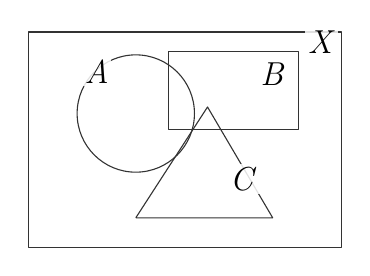
\begin{tikzpicture}[line join=round]
\filldraw[draw=black!80,fill=none] (0.515,-3.247) rectangle (4.489,-0.515);
\draw[black!80] (1.881,-1.550) circle (0.745);
\filldraw[draw=black!80,fill=none] (2.295,-1.757) rectangle (3.951,-0.763);
\draw[black!80] (1.881,-2.875) -- (3.620,-2.875) -- (2.792,-1.467) -- (1.881,-2.875);
\node[fill=white,fill opacity=0.85,text opacity=1,inner sep=1pt,font=\large] at (1.384,-1.012) {\textit{A}};
\node[fill=white,fill opacity=0.85,text opacity=1,inner sep=1pt,font=\large] at (3.620,-1.053) {\textit{B}};
\node[fill=white,fill opacity=0.85,text opacity=1,inner sep=1pt,font=\large] at (3.247,-2.378) {\textit{C}};
\node[fill=white,fill opacity=0.85,text opacity=1,inner sep=1pt,font=\large] at (4.241,-0.639) {\textit{X}};
\end{tikzpicture}\par\smallskip{\small\raggedright \textbf{Three overlapping subsets of \textit{X}.} The outlines show the regions named by \textit{A}, \textit{B} and \textit{C}; the membership tests below specify exactly which points each answer keeps.\par}\end{minipage}
\end{center}

\nopagebreak[4]{\small\itshape Answers: see “Exercise 1.2: Sets” under Answers at the end.}
\end{keepsection}

\begin{keepsection}
\Needspace{7\baselineskip}
\subsection{2b: Work with even, odd and ordered-pair sets}

\Needspace{4\baselineskip}
Try first: separate the integer examples from the ordered-pair example, and check both coordinates of each pair.

\nopagebreak[4]{\small\itshape Answers: see “Exercise 1.2: Sets” under Answers at the end.}
\end{keepsection}

\begin{keepsection}
\Needspace{7\baselineskip}
\subsection{2c: Prove a set identity by membership}

\Needspace{4\baselineskip}
Try first: take an arbitrary \textit{x} and translate both “set difference” steps into and/not conditions.

\nopagebreak[4]{\small\itshape Answers: see “Exercise 1.2: Sets” under Answers at the end.}
\end{keepsection}
\end{keepsection}

\begin{keepsection}
\Needspace{9\baselineskip}
\section{Exercise 1.3: Quantifiers — students and courses}

\Needspace{6\baselineskip}
Let \textit{S} be the student set, \textit{C} the course set, and \textit{B}(\textit{s}, \textit{c}) mean that student \textit{s} passed course \textit{c}. The order of “for all” and “there exists” determines who may vary.

\textbf{Connected topic:} Predicates, quantifier order and negation (§1.1) define the domain and the order in which choices are made.

\begin{keepsection}
\Needspace{7\baselineskip}
\subsection{3a: Translate “a bright spark passes everything”}

\Needspace{4\baselineskip}
Try first: decide whether the student is chosen before or after the course, and whether one student must pass every course.

\nopagebreak[4]{\small\itshape Answers: see “Exercise 1.3: Quantifiers — students and courses” under Answers at the end.}
\end{keepsection}

\begin{keepsection}
\Needspace{7\baselineskip}
\subsection{3b: Translate “nobody passed the whole programme”}

\Needspace{4\baselineskip}
Try first: negate “there is a student who passed every course”, then swap the quantifiers as you push the negation inward.

\nopagebreak[4]{\small\itshape Answers: see “Exercise 1.3: Quantifiers — students and courses” under Answers at the end.}
\end{keepsection}

\begin{keepsection}
\Needspace{7\baselineskip}
\subsection{3c: Translate “a course everyone passes”}

\Needspace{4\baselineskip}
Try first: identify the one course that must work for every student, then contrast it with “each student has some course”.

\nopagebreak[4]{\small\itshape Answers: see “Exercise 1.3: Quantifiers — students and courses” under Answers at the end.}
\end{keepsection}
\end{keepsection}

\begin{keepsection}
\Needspace{9\baselineskip}
\section{Self-Study 1.4: Statements}

\Needspace{6\baselineskip}
This review combines statement classification, truth tables, implication language and translating ordinary “unless” sentences.

\textbf{Connected topic:} Statements, truth tables and logical equivalence (§1.1) define the tests used below.

\begin{keepsection}
\Needspace{7\baselineskip}
\subsection{4a: Decide whether each sentence is a statement}

\Needspace{4\baselineskip}
Try first: check whether the sentence asserts something with a definite truth value, not whether you personally know the value.

\nopagebreak[4]{\small\itshape Answers: see “Self-Study 1.4: Statements” under Answers at the end.}
\end{keepsection}

\begin{keepsection}
\Needspace{7\baselineskip}
\subsection{4b: Verify two equivalences by truth table}

\Needspace{4\baselineskip}
Try first: make one table for the distributive law and a second for De Morgan’s law; compare the two target columns row by row.

\nopagebreak[4]{\small\itshape Answers: see “Self-Study 1.4: Statements” under Answers at the end.}
\end{keepsection}

\begin{keepsection}
\Needspace{6\baselineskip}
\subsection{4c: Rewrite “if” and “only if” sentences}

\Needspace{3\baselineskip}
Try first: for “\textit{X} only if \textit{Y}”, write \textit{X} \ensuremath{\Rightarrow} \textit{Y}; then substitute the given truth values.

\nopagebreak[4]{\small\itshape Answers: see “Self-Study 1.4: Statements” under Answers at the end.}
\end{keepsection}

\begin{keepsection}
\Needspace{6\baselineskip}
\subsection{4d: Show that a conditional is not a tautology}

\Needspace{3\baselineskip}
Try first: to make an implication false, make its antecedent true and its consequent false.

\nopagebreak[4]{\small\itshape Answers: see “Self-Study 1.4: Statements” under Answers at the end.}
\end{keepsection}

\begin{keepsection}
\Needspace{7\baselineskip}
\subsection{4e: Translate “if”, “only if” and “unless”}

\Needspace{4\baselineskip}
Try first: “\textit{B} unless \textit{G}” means that if \textit{G} is absent, \textit{B} does not happen. Compare the directions after translating.

\nopagebreak[4]{\small\itshape Answers: see “Self-Study 1.4: Statements” under Answers at the end.}
\end{keepsection}
\end{keepsection}

\begin{keepsection}
\Needspace{9\baselineskip}
\section{Self-Study 1.5: Sets}

\Needspace{6\baselineskip}
Use the intervals and point set in the source diagram. Complements here are relative to \ensuremath{\mathbb{R}}, since the exercise defines all three sets as subsets of \ensuremath{\mathbb{R}}.

\textbf{Connected topic:} Intervals, complements and power sets (§1.2) define membership and the universe for these operations.

\begin{keepsection}
\Needspace{12\baselineskip}
\subsection{5a: Combine two intervals with a finite set}

\Needspace{9\baselineskip}
Try first: write the sets as \textit{A} = (\ensuremath{-}2, 1], \textit{B} = (\ensuremath{-}1, 1), and \textit{C} = \{\ensuremath{-}2, 0, 1\}; mark the endpoints before combining.

\Needspace{14\baselineskip}
\begin{center}
\begin{minipage}[t]{0.303\linewidth}\centering
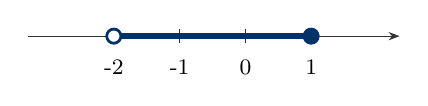
\begin{tikzpicture}[line join=round]
\draw[-{Stealth[length=4pt]},black!80] (0.180,-0.612) -- (4.896,-0.612);
\draw[black!80] (1.267,-0.522) -- (1.267,-0.702);
\node[,inner sep=1pt,font=\footnotesize] at (1.267,-1.008) {-2};
\draw[black!80] (2.102,-0.522) -- (2.102,-0.702);
\node[,inner sep=1pt,font=\footnotesize] at (2.102,-1.008) {-1};
\draw[black!80] (2.938,-0.522) -- (2.938,-0.702);
\node[,inner sep=1pt,font=\footnotesize] at (2.938,-1.008) {0};
\draw[black!80] (3.773,-0.522) -- (3.773,-0.702);
\node[,inner sep=1pt,font=\footnotesize] at (3.773,-1.008) {1};
\draw[FAUblue,line width=2.2pt] (1.267,-0.612) -- (3.773,-0.612);
\filldraw[draw=FAUblue,fill=white,line width=1pt] (1.267,-0.612) circle (0.090);
\filldraw[draw=FAUblue,fill=FAUblue,line width=1pt] (3.773,-0.612) circle (0.090);
\end{tikzpicture}\par\smallskip{\small\raggedright \textbf{\textit{A} = (\ensuremath{-}2, 1].} The left endpoint is open and the right endpoint is included.\par}\end{minipage}\hfill
\begin{minipage}[t]{0.303\linewidth}\centering
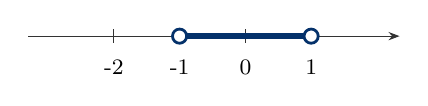
\begin{tikzpicture}[line join=round]
\draw[-{Stealth[length=4pt]},black!80] (0.180,-0.612) -- (4.896,-0.612);
\draw[black!80] (1.267,-0.522) -- (1.267,-0.702);
\node[,inner sep=1pt,font=\footnotesize] at (1.267,-1.008) {-2};
\draw[black!80] (2.102,-0.522) -- (2.102,-0.702);
\node[,inner sep=1pt,font=\footnotesize] at (2.102,-1.008) {-1};
\draw[black!80] (2.938,-0.522) -- (2.938,-0.702);
\node[,inner sep=1pt,font=\footnotesize] at (2.938,-1.008) {0};
\draw[black!80] (3.773,-0.522) -- (3.773,-0.702);
\node[,inner sep=1pt,font=\footnotesize] at (3.773,-1.008) {1};
\draw[FAUblue,line width=2.2pt] (2.102,-0.612) -- (3.773,-0.612);
\filldraw[draw=FAUblue,fill=white,line width=1pt] (2.102,-0.612) circle (0.090);
\filldraw[draw=FAUblue,fill=white,line width=1pt] (3.773,-0.612) circle (0.090);
\end{tikzpicture}\par\smallskip{\small\raggedright \textbf{\textit{B} = (\ensuremath{-}1, 1).} Both endpoints are excluded.\par}\end{minipage}\hfill
\begin{minipage}[t]{0.303\linewidth}\centering
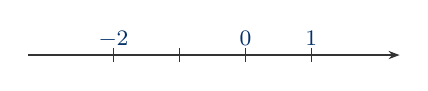
\begin{tikzpicture}[line join=round]
\draw[-{Stealth[length=4pt]},black!80] (0.180,-0.612) -- (4.896,-0.612);
\draw[black!80] (1.267,-0.522) -- (1.267,-0.702);
\draw[black!80] (2.102,-0.522) -- (2.102,-0.702);
\draw[black!80] (2.938,-0.522) -- (2.938,-0.702);
\draw[black!80] (3.773,-0.522) -- (3.773,-0.702);
\node[text=FAUblue,inner sep=1pt,font=\footnotesize] at (1.267,-0.396) {\ensuremath{-}2};
\node[text=FAUblue,inner sep=1pt,font=\footnotesize] at (2.938,-0.396) {0};
\node[text=FAUblue,inner sep=1pt,font=\footnotesize] at (3.773,-0.396) {1};
\end{tikzpicture}\par\smallskip{\small\raggedright \textbf{\textit{C} = \{\ensuremath{-}2, 0, 1\}.} The red points mark the three roots of \textit{x}(\textit{x} + 2)(\textit{x} \ensuremath{-} 1) = 0.\par}\end{minipage}
\end{center}

\nopagebreak[4]{\small\itshape Answers: see “Self-Study 1.5: Sets” under Answers at the end.}
\end{keepsection}

\begin{keepsection}
\Needspace{7\baselineskip}
\subsection{5b: Form two power sets and test membership}

\Needspace{4\baselineskip}
Try first: list subsets by size, and expand the Cartesian product before deciding what its power set contains.

\nopagebreak[4]{\small\itshape Answers: see “Self-Study 1.5: Sets” under Answers at the end.}
\end{keepsection}

\begin{keepsection}
\Needspace{6\baselineskip}
\subsection{5c: Prove a difference identity}

\Needspace{3\baselineskip}
Try first: expand “not in \textit{B} \textbackslash{} \textit{C}” and distribute “and” over “or”.

\nopagebreak[4]{\small\itshape Answers: see “Self-Study 1.5: Sets” under Answers at the end.}
\end{keepsection}
\end{keepsection}

\begin{keepsection}
\Needspace{9\baselineskip}
\section{Self-Study 1.6: Quantifiers and numbers}

\Needspace{6\baselineskip}
For each domain, decide whether every quantified claim holds. In these notes, \ensuremath{\mathbb{N}} = \{1, 2, 3, …\}, \ensuremath{\mathbb{Z}} is the integers, and \ensuremath{\mathbb{R}}\textsuperscript{+} = (0, \ensuremath{\infty}).

\textbf{Connected topics:} Quantifiers and negation (§1.1) and number systems (§2.1) specify the logic and the three domains.

\begin{keepsection}
\Needspace{7\baselineskip}
\subsection{6a: Evaluate four statements and write their negations}

\Needspace{4\baselineskip}
Try first: substitute a test value to disprove a universal claim; to prove one, give a valid witness for every value required.

\nopagebreak[4]{\small\itshape Answers: see “Self-Study 1.6: Quantifiers and numbers” under Answers at the end.}
\end{keepsection}
\end{keepsection}


\clearpage
\section{Answers}
\begin{keepsection}\subsection{Exercise 1.1: Statements}

\begin{workedbox}{1a \ensuremath{\cdot} A definite truth value}
\Needspace{15\baselineskip}
\begin{enumerate}
\item \textbf{i. “\textit{z} is prime.”} The value of \textit{z} has not been given or quantified. This is an open form: it becomes a statement only after a value is assigned to \textit{z} (or a quantifier is added). \textbf{As written, it is not a statement.}
\item \textbf{ii. The claim about Lothar Matthäus and the 2011 Tour de France.} It names a particular person and event, with no free variable. It is a factual declarative sentence, so it has a definite truth value whether or not the reader knows it. \textbf{It is a statement.}
\item \textbf{iii. “This statement is false.”} If it were true, what it says would make it false; if it were false, then what it says would be true. It cannot be assigned a consistent true-or-false value in ordinary two-valued logic. \textbf{It is not a logical statement.}
\item \textbf{iv. The conditional involving \textit{n} and the oak trees.} The variable \textit{n} is free, so different values of \textit{n} can change the antecedent. The sentence would need a specified \textit{n}, or a quantifier such as “for every \textit{n}”. \textbf{As written, it is not a statement.}
\end{enumerate}
\end{workedbox}

\end{keepsection}
\begin{keepsection}\subsection{Exercise 1.1: Statements}

\begin{workedbox}{1b \ensuremath{\cdot} Truth table for implication and its contrapositive}
\Needspace{11\baselineskip}
\begin{enumerate}
\item There are two propositions, so there are four input rows. In the last column, the three expressions are linked by biconditionals; that column is true when their truth values agree.
\item \Needspace{10\baselineskip}
\begin{center}\small\begin{tabularx}{\linewidth}{>{\raggedright\arraybackslash}X>{\raggedright\arraybackslash}X>{\raggedright\arraybackslash}X>{\raggedright\arraybackslash}X>{\raggedright\arraybackslash}X>{\raggedright\arraybackslash}X}\toprule
\textbf{\textit{A}} & \textbf{\textit{B}} & \textbf{\textit{A} \ensuremath{\Rightarrow} \textit{B}} & \textbf{\ensuremath{\neg}\textit{B} \ensuremath{\Rightarrow} \ensuremath{\neg}\textit{A}} & \textbf{\ensuremath{\neg}(\textit{A} \ensuremath{\land} \ensuremath{\neg}\textit{B})} & \textbf{whole chain} \\ \midrule
T & T & T & T & T & T \\
T & F & F & F & F & T \\
F & T & T & T & T & T \\
F & F & T & T & T & T \\
\bottomrule\end{tabularx}\end{center}
\item The columns for \textit{A} \ensuremath{\Rightarrow} \textit{B}, \ensuremath{\neg}\textit{B} \ensuremath{\Rightarrow} \ensuremath{\neg}\textit{A}, and \ensuremath{\neg}(\textit{A} \ensuremath{\land} \ensuremath{\neg}\textit{B}) match in every row. The biconditional chain is therefore true in all four rows: all three formulas are equivalent, and the chain is a tautology.
\item \textbf{Check by rules:} \ensuremath{\neg}\textit{B} \ensuremath{\Rightarrow} \ensuremath{\neg}\textit{A} is the contrapositive of \textit{A} \ensuremath{\Rightarrow} \textit{B}. Also, implication is equivalent to \ensuremath{\neg}\textit{A} \ensuremath{\lor} \textit{B}, and De Morgan’s law gives \ensuremath{\neg}(\textit{A} \ensuremath{\land} \ensuremath{\neg}\textit{B}) = \ensuremath{\neg}\textit{A} \ensuremath{\lor} \textit{B}.
\end{enumerate}
\end{workedbox}

\end{keepsection}
\begin{keepsection}\subsection{Exercise 1.1: Statements}

\begin{workedbox}{1c \ensuremath{\cdot} Translate the clues and eliminate cases}
\Needspace{13\baselineskip}
\begin{enumerate}
\item \Needspace{5\baselineskip}
Let \textit{A}, \textit{B} and \textit{C} mean that Anton, Bert and Christoph, respectively, are guilty. The three clues become:

\Needspace{4\baselineskip}
\begin{equation*}{C}\, \Rightarrow \, {A}\end{equation*}

\Needspace{4\baselineskip}
\begin{equation*}({B}\, \lor \, {C})\, \Rightarrow \, \neg {A}\end{equation*}

\begin{equation*}(\neg {A}\, \lor \, \neg {C})\, \Rightarrow \, {B}\end{equation*}
\item Suppose \textit{C} were true. The first clue would make \textit{A} true. Then \textit{B} \ensuremath{\lor} \textit{C} is true, so the second clue makes \ensuremath{\neg}\textit{A} true. That contradicts \textit{A}; hence \textit{C} is false.
\item Because \ensuremath{\neg}\textit{C} is true, the antecedent \textit{A} \ensuremath{\lor} \ensuremath{\neg}\textit{C} in the third clue is true. Therefore \textit{B} is true: Bert is guilty.
\item Now \textit{B} \ensuremath{\lor} \textit{C} is true, so the second clue gives \ensuremath{\neg}\textit{A}. Anton is innocent, and we already found Christoph innocent.
\item \textbf{Conclusion:} \textit{B} is true while \textit{A} and \textit{C} are false. \textbf{Bert committed the crime.} Substitution checks all three clues: true, true, and true.
\end{enumerate}
\end{workedbox}

\end{keepsection}
\begin{keepsection}\subsection{Exercise 1.2: Sets}

\begin{workedbox}{2a \ensuremath{\cdot} Convert each expression to a membership test}
\Needspace{16\baselineskip}
\begin{enumerate}
\item \Needspace{5\baselineskip}
For i), membership in \textit{A} \textbackslash{} \textit{B} means “in \textit{A} and not in \textit{B}”. Intersecting with \textit{C} adds one more “and”:

\Needspace{4\baselineskip}
\begin{equation*}{x}\, \in \, ({A}\, \\, {B})\, \cap \, {C}\, \Leftrightarrow \, ({x}\, \in \, {A})\, \land \, ({x}\, \notin \, {B})\, \land \, ({x}\, \in \, {C})\end{equation*}

Keep the part shared by \textit{A} and \textit{C} that lies outside \textit{B}.
\item \Needspace{5\baselineskip}
For ii), union means “or”. Keep every point in \textit{C}, together with any point that is in \textit{A} but outside \textit{B}:

\begin{equation*}{x}\, \in \, ({A}\, \\, {B})\, \cup \, {C}\, \Leftrightarrow \, (({x}\, \in \, {A})\, \land \, ({x}\, \notin \, {B}))\, \lor \, ({x}\, \in \, {C})\end{equation*}
\item \Needspace{5\baselineskip}
For iii), a complement keeps the points in \textit{X} that fail membership in the whole union. De Morgan’s law changes “not (P or Q)” to “not P and not Q”:

\Needspace{4\baselineskip}
\begin{equation*}(({A}\, \\, {B})\, \cup \, {C})^{\mathrm{c}}\, =\, (({A}\, \\, {B})^{\mathrm{c}})\, \cap \, {C}^{\mathrm{c}}\, =\, ({A}^{\mathrm{c}}\, \cup \, {B})\, \cap \, {C}^{\mathrm{c}}\end{equation*}

So keep points outside \textit{C} and either outside \textit{A} or inside \textit{B}.
\item \Needspace{5\baselineskip}
For iv), first combine the two differences: \textit{A} \textbackslash{} \textit{C} and \textit{B} \textbackslash{} \textit{C} together are all of \textit{A} \ensuremath{\cup} \textit{B} with \textit{C} removed. Complementing adds \textit{C} back and keeps the points outside both \textit{A} and \textit{B}:

\begin{equation*}(({A}\, \\, {C})\, \cup \, ({B}\, \\, {C}))^{\mathrm{c}}\, =\, (({A}\, \cup \, {B})\, \\, {C})^{\mathrm{c}}\, =\, ({A}\, \cup \, {B})^{\mathrm{c}}\, \cup \, {C}\end{equation*}
\item \textbf{Check:} in iii) any point inside \textit{C} is excluded; in iv) every point inside \textit{C} is included. That opposite treatment is a quick way to catch a misplaced complement.
\end{enumerate}
\end{workedbox}

\end{keepsection}
\begin{keepsection}\subsection{Exercise 1.2: Sets}

\begin{workedbox}{2b \ensuremath{\cdot} Operations, products and power sets}
\Needspace{12\baselineskip}
\begin{enumerate}
\item \Needspace{5\baselineskip}
\textit{A} contains the positive even natural numbers; \textit{B} contains the positive odd natural numbers. Every positive natural number is exactly one of these, so:

\Needspace{4\baselineskip}
\begin{equation*}{A}\, \cup \, {B}\, =\, \mathbb{N}\end{equation*}

\Needspace{4\baselineskip}
\begin{equation*}{A}\, \cap \, {B}\, =\, \emptyset \end{equation*}

\Needspace{4\baselineskip}
\begin{equation*}{A}\, \\, {B}\, =\, {A}\end{equation*}

\begin{equation*}{B}\, \\, {A}\, =\, {B}\end{equation*}
\item \Needspace{5\baselineskip}
The Cartesian product asks for ordered pairs whose first entry is in the first factor and second entry is in the second:

\begin{equation*}{A}\, \times \, {B}\, =\, \{({a},\, {b})\, :\, {a}\, \in \, {A},\, {b}\, \in \, {B}\}\end{equation*}
\item Test the two elements of \textit{C} separately. (\textit{2}, \textit{3}) passes: 2 is even and 3 is odd. (\textit{3}, \textit{4}) fails: 3 is not even and 4 is not odd. Since one element fails, \textbf{\textit{C} is not a subset of \textit{A} \ensuremath{\times} \textit{B}.}
\item \Needspace{5\baselineskip}
The power set contains every subset of \textit{C}: the empty set, each one-element subset, and \textit{C} itself.

\Needspace{4\baselineskip}
\begin{equation*}\mathcal{P}({C})\, =\, \{\emptyset ,\, \{({2},\, {3})\},\, \{({3},\, {4})\},\, \{({2},\, {3}),\, ({3},\, {4})\}\}\end{equation*}

There are 2² = 4 subsets, matching the two elements of \textit{C}.
\end{enumerate}
\end{workedbox}

\end{keepsection}
\begin{keepsection}\subsection{Exercise 1.2: Sets}

\begin{workedbox}{2c \ensuremath{\cdot} Element-by-element proof}
\Needspace{11\baselineskip}
\begin{enumerate}
\item \Needspace{4\baselineskip}
Take any \textit{x}. It belongs to the left-hand side exactly when it is in \textit{A} but not in \textit{A} \textbackslash{} \textit{B}:

\begin{equation*}{x}\, \in \, {A}\, \\, ({A}\, \\, {B})\, \Leftrightarrow \, ({x}\, \in \, {A})\, \land \, \neg ({x}\, \in \, {A}\, \\, {B})\end{equation*}
\item \Needspace{4\baselineskip}
Expand the inner difference: \textit{x} \ensuremath{\in} \textit{A} \textbackslash{} \textit{B} means \textit{x} \ensuremath{\in} \textit{A} and \textit{x} \ensuremath{\notin} \textit{B}. Therefore:

\begin{equation*}({x}\, \in \, {A})\, \land \, \neg (({x}\, \in \, {A})\, \land \, ({x}\, \notin \, {B}))\end{equation*}
\item \Needspace{5\baselineskip}
Because we already know \textit{x} \ensuremath{\in} \textit{A}, the negated inner condition reduces to \textit{x} \ensuremath{\in} \textit{B}. Thus membership is equivalent to \textit{x} \ensuremath{\in} \textit{A} and \textit{x} \ensuremath{\in} \textit{B}:

\begin{equation*}{x}\, \in \, {A}\, \\, ({A}\, \\, {B})\, \Leftrightarrow \, {x}\, \in \, {A}\, \cap \, {B}\end{equation*}
\item This is true for every \textit{x}, so both sets contain exactly the same elements. Hence \textbf{\textit{A} \textbackslash{} (\textit{A} \textbackslash{} \textit{B}) = \textit{A} \ensuremath{\cap} \textit{B}.}
\end{enumerate}
\end{workedbox}

\end{keepsection}
\begin{keepsection}\subsection{Exercise 1.3: Quantifiers — students and courses}

\begin{workedbox}{3a \ensuremath{\cdot} One student, all courses}
\Needspace{10\baselineskip}
\begin{enumerate}
\item “There is a student” gives \ensuremath{\exists}\textit{s}. “Passes everything” says that same student passes every course, giving \ensuremath{\forall}\textit{c}. The correct choice is \textbf{b) \ensuremath{\exists}\textit{s} \ensuremath{\in} \textit{S} \ensuremath{\forall}\textit{c} \ensuremath{\in} \textit{C}: \textit{B}(\textit{s}, \textit{c}).}
\item \Needspace{11\baselineskip}
Translate the other choices to see the difference:

\Needspace{10\baselineskip}
\begin{center}\small\begin{tabularx}{\linewidth}{>{\raggedright\arraybackslash}X>{\raggedright\arraybackslash}X}\toprule
\textbf{Choice} & \textbf{Meaning} \\ \midrule
a) \ensuremath{\forall}\textit{s} \ensuremath{\exists}\textit{c} \textit{B}(\textit{s},\textit{c}) & Every student has passed at least one course; it may be a different course for each student. \\
c) \ensuremath{\exists}\textit{s} \ensuremath{\exists}\textit{c} \textit{B}(\textit{s},\textit{c}) & At least one student has passed at least one course. \\
d) \ensuremath{\forall}\textit{c} \ensuremath{\exists}\textit{s} \textit{B}(\textit{s},\textit{c}) & Every course has at least one student who passed it; the student may vary by course. \\
\bottomrule\end{tabularx}\end{center}
\item \textbf{Check:} \ensuremath{\exists}\textit{s}\ensuremath{\forall}\textit{c} is stronger than \ensuremath{\forall}\textit{s}\ensuremath{\exists}\textit{c}. The former fixes one student and then asks about every course.
\end{enumerate}
\end{workedbox}

\end{keepsection}
\begin{keepsection}\subsection{Exercise 1.3: Quantifiers — students and courses}

\begin{workedbox}{3b \ensuremath{\cdot} Each student missed a course}
\Needspace{12\baselineskip}
\begin{enumerate}
\item \Needspace{4\baselineskip}
“Nobody has made it through” means there is no student who passed all courses:

\begin{equation*}\neg (\exists {s}\, \in \, {S}\, \forall {c}\, \in \, {C}:\, {B}({s},\, {c}))\end{equation*}
\item \Needspace{4\baselineskip}
Negating \ensuremath{\exists} changes it to \ensuremath{\forall}; negating \ensuremath{\forall} changes it to \ensuremath{\exists}; the predicate is negated too:

\Needspace{4\baselineskip}
\begin{equation*}\forall {s}\, \in \, {S}\, \exists {c}\, \in \, {C}:\, \neg {B}({s},\, {c})\end{equation*}

So the answer is \textbf{d)}: every student has at least one course they have not passed.
\item \Needspace{10\baselineskip}
The other options say:

\Needspace{10\baselineskip}
\begin{center}\small\begin{tabularx}{\linewidth}{>{\raggedright\arraybackslash}X>{\raggedright\arraybackslash}X}\toprule
\textbf{Choice} & \textbf{Meaning} \\ \midrule
a) \ensuremath{\exists}\textit{s} \ensuremath{\forall}\textit{c} \ensuremath{\neg}\textit{B}(\textit{s},\textit{c}) & At least one student has passed no courses. \\
b) \ensuremath{\forall}\textit{c} \ensuremath{\exists}\textit{s} \ensuremath{\neg}\textit{B}(\textit{s},\textit{c}) & Every course has at least one student who has not passed it. \\
c) \ensuremath{\forall}\textit{s} \ensuremath{\forall}\textit{c} \ensuremath{\neg}\textit{B}(\textit{s},\textit{c}) & No student has passed any course. \\
\bottomrule\end{tabularx}\end{center}
\item \textbf{Check:} the correct statement allows a student to have passed most courses; it only requires one unpassed course for each student.
\end{enumerate}
\end{workedbox}

\end{keepsection}
\begin{keepsection}\subsection{Exercise 1.3: Quantifiers — students and courses}

\begin{workedbox}{3c \ensuremath{\cdot} One course, all students}
\Needspace{9\baselineskip}
\begin{enumerate}
\item “There is a course” gives \ensuremath{\exists}\textit{c}; “every student passes it” gives \ensuremath{\forall}\textit{s}. The correct choice is \textbf{a) \ensuremath{\exists}\textit{c} \ensuremath{\in} \textit{C} \ensuremath{\forall}\textit{s} \ensuremath{\in} \textit{S}: \textit{B}(\textit{s}, \textit{c}).}
\item \Needspace{10\baselineskip}
The other formulas mean:

\Needspace{10\baselineskip}
\begin{center}\small\begin{tabularx}{\linewidth}{>{\raggedright\arraybackslash}X>{\raggedright\arraybackslash}X}\toprule
\textbf{Choice} & \textbf{Meaning} \\ \midrule
b) \ensuremath{\forall}\textit{c} \ensuremath{\exists}\textit{s} \textit{B}(\textit{s},\textit{c}) & Every course has some student who passed it. \\
c) \ensuremath{\forall}\textit{s} \ensuremath{\exists}\textit{c} \textit{B}(\textit{s},\textit{c}) & Every student has passed at least one course. \\
d) \ensuremath{\exists}\textit{s} \ensuremath{\forall}\textit{c} \textit{B}(\textit{s},\textit{c}) & Some student has passed every course. \\
\bottomrule\end{tabularx}\end{center}
\item \textbf{Check:} in a), one course is chosen first and then tested for every student. In d), it is one student tested against every course.
\end{enumerate}
\end{workedbox}

\end{keepsection}
\begin{keepsection}\subsection{Self-Study 1.4: Statements}

\begin{workedbox}{4a \ensuremath{\cdot} Assertion or open judgement?}
\Needspace{8\baselineskip}
\begin{enumerate}
\item \textbf{i. The conditional about a father having a sibling.} It is a complete declarative sentence with a fixed family relation as its subject. It can be true or false, even if the family facts are unknown. \textbf{It is a statement.}
\item \textbf{ii. “The formula is beautiful.”} No formula or precise criterion for “beautiful” is specified. Under the guide’s logical definition, the sentence has no definite truth value. \textbf{As written, it is not a logical statement.}
\end{enumerate}
\end{workedbox}

\end{keepsection}
\begin{keepsection}\subsection{Self-Study 1.4: Statements}

\begin{workedbox}{4b \ensuremath{\cdot} Distributive law and De Morgan’s law}
\Needspace{12\baselineskip}
\begin{enumerate}
\item \Needspace{15\baselineskip}
For i), evaluate the left side \textit{A} \ensuremath{\land} (\textit{B} \ensuremath{\lor} \textit{C}) and right side (\textit{A} \ensuremath{\land} \textit{B}) \ensuremath{\lor} (\textit{A} \ensuremath{\land} \textit{C}) for all eight assignments:

\Needspace{10\baselineskip}
\begin{center}\small\begin{tabularx}{\linewidth}{>{\raggedright\arraybackslash}X>{\raggedright\arraybackslash}X>{\raggedright\arraybackslash}X>{\raggedright\arraybackslash}X>{\raggedright\arraybackslash}X}\toprule
\textbf{\textit{A}} & \textbf{\textit{B}} & \textbf{\textit{C}} & \textbf{\textit{A} \ensuremath{\land} (\textit{B} \ensuremath{\lor} \textit{C})} & \textbf{(\textit{A} \ensuremath{\land} \textit{B}) \ensuremath{\lor} (\textit{A} \ensuremath{\land} \textit{C})} \\ \midrule
T & T & T & T & T \\
T & T & F & T & T \\
T & F & T & T & T \\
T & F & F & F & F \\
F & T & T & F & F \\
F & T & F & F & F \\
F & F & T & F & F \\
F & F & F & F & F \\
\bottomrule\end{tabularx}\end{center}
\item The two columns agree in all eight rows, so the distributive equivalence is true for every assignment.
\item \Needspace{10\baselineskip}
For ii), compare both sides of \ensuremath{\neg}(\textit{A} \ensuremath{\land} \textit{B}) \ensuremath{\Leftrightarrow} \ensuremath{\neg}\textit{A} \ensuremath{\lor} \ensuremath{\neg}\textit{B}:

\Needspace{10\baselineskip}
\begin{center}\small\begin{tabularx}{\linewidth}{>{\raggedright\arraybackslash}X>{\raggedright\arraybackslash}X>{\raggedright\arraybackslash}X>{\raggedright\arraybackslash}X}\toprule
\textbf{\textit{A}} & \textbf{\textit{B}} & \textbf{\ensuremath{\neg}(\textit{A} \ensuremath{\land} \textit{B})} & \textbf{\ensuremath{\neg}\textit{A} \ensuremath{\lor} \ensuremath{\neg}\textit{B}} \\ \midrule
T & T & F & F \\
T & F & T & T \\
F & T & T & T \\
F & F & T & T \\
\bottomrule\end{tabularx}\end{center}
\item These columns also agree in every row. The equivalence is a tautology, which verifies this De Morgan law.
\end{enumerate}
\end{workedbox}

\end{keepsection}
\begin{keepsection}\subsection{Self-Study 1.4: Statements}

\begin{workedbox}{4c \ensuremath{\cdot} Conditional direction and truth value}
\Needspace{15\baselineskip}
\begin{enumerate}
\item Use \textit{C} = cats have wings, \textit{D} = dogs have wings, \textit{P} = parrots have wings. The given assignment makes all three false.
\item \textbf{i. Cats have wings only if dogs have wings.} “Only if” puts the necessary condition second: \textit{C} \ensuremath{\Rightarrow} \textit{D}, read “If cats have wings, then dogs have wings.” It is true because the antecedent \textit{C} is false.
\item \textbf{ii. Parrots have wings only if dogs have wings.} Formula \textit{P} \ensuremath{\Rightarrow} \textit{D}, read “If parrots have wings, then dogs have wings.” It is true because \textit{P} is false.
\item \textbf{iii. Parrots have wings if dogs have wings.} The condition after “if” is the antecedent: \textit{D} \ensuremath{\Rightarrow} \textit{P}, read “If dogs have wings, then parrots have wings.” It is true because \textit{D} is false.
\item \textbf{iv. If cats or dogs have wings, then both cats and dogs have wings.} Formula (\textit{C} \ensuremath{\lor} \textit{D}) \ensuremath{\Rightarrow} (\textit{C} \ensuremath{\land} \textit{D}). It is true because its antecedent is false. \textbf{All four sentences are true} for the supplied assignment; a conditional with a false antecedent is true in the truth-table definition.
\end{enumerate}
\end{workedbox}

\end{keepsection}
\begin{keepsection}\subsection{Self-Study 1.4: Statements}

\begin{workedbox}{4d \ensuremath{\cdot} One counterexample is enough}
\Needspace{7\baselineskip}
\begin{enumerate}
\item Choose \textit{A} = false and \textit{B} = true. Then \textit{A} \ensuremath{\Rightarrow} \textit{B} is true (false antecedent), while \textit{B} \ensuremath{\Rightarrow} \textit{A} is false (true antecedent and false consequent).
\item \Needspace{4\baselineskip}
The outer implication is therefore true \ensuremath{\Rightarrow} false, which is false:

\begin{equation*}({A}\, \Rightarrow \, {B})\, \Rightarrow \, ({B}\, \Rightarrow \, {A})\, =\, \mathrm{T}\, \Rightarrow \, \mathrm{F}\, =\, \mathrm{F}\end{equation*}
\item A tautology must be true for every assignment. This single false row proves the formula is \textbf{not} a tautology.
\end{enumerate}
\end{workedbox}

\end{keepsection}
\begin{keepsection}\subsection{Self-Study 1.4: Statements}

\begin{workedbox}{4e \ensuremath{\cdot} Mirror conditions}
\Needspace{13\baselineskip}
\begin{enumerate}
\item Let \textit{B} mean the mirror breaks, \textit{G} mean it is made of glass, and \textit{W} mean it is high on the wall.
\item \textbf{i. Breaks if it is made of glass:} glass is sufficient for breaking, so \textit{G} \ensuremath{\Rightarrow} \textit{B}.
\item \textbf{ii. Breaks only if it is made of glass:} glass is necessary for breaking, so \textit{B} \ensuremath{\Rightarrow} \textit{G}.
\item \textbf{iii. Unless it is made of glass, it will not break:} if it is not glass, it does not break: \ensuremath{\neg}\textit{G} \ensuremath{\Rightarrow} \ensuremath{\neg}\textit{B}. By contraposition, this is equivalent to \textit{B} \ensuremath{\Rightarrow} \textit{G}.
\item \textbf{iv. It is high on the wall, but will not break unless it is glass:} “but” is conjunction, so the full formula is \textit{W} \ensuremath{\land} (\ensuremath{\neg}\textit{G} \ensuremath{\Rightarrow} \ensuremath{\neg}\textit{B}), equivalently \textit{W} \ensuremath{\land} (\textit{B} \ensuremath{\Rightarrow} \textit{G}).
\item \textbf{Equivalent pair:} ii) and iii) express the same conditional. In iv), that conditional is joined to the extra requirement \textit{W}, so iv) is not generally equivalent to ii).
\end{enumerate}
\end{workedbox}

\end{keepsection}
\begin{keepsection}\subsection{Self-Study 1.5: Sets}

\begin{workedbox}{5a \ensuremath{\cdot} Intervals and roots}
\Needspace{17\baselineskip}
\begin{enumerate}
\item Factor equation \textit{x}(\textit{x} + 2)(\textit{x} \ensuremath{-} 1) = 0. A product is zero when a factor is zero, so \textit{C} = \{\ensuremath{-}2, 0, 1\}. The interval \textit{B} sits entirely inside \textit{A}.
\item \textit{A} \ensuremath{\cap} \textit{B} keeps numbers in both. Since \textit{B} is contained in \textit{A}, the answer is \textbf{(\ensuremath{-}1, 1).}
\item \textit{A} \ensuremath{\cap} \textit{B} \ensuremath{\cap} \textit{C} asks which listed roots lie in the overlap (\ensuremath{-}1, 1). Only 0 does, so the answer is \textbf{\{0\}.}
\item \textit{A} \ensuremath{\cap} (\textit{B} \ensuremath{\cup} \textit{C}) starts with \textit{B} \ensuremath{\cap} \textit{A} = (\ensuremath{-}1, 1). Of the points in \textit{C}, 0 is already there, 1 belongs to \textit{A}, and \ensuremath{-}2 does not. Thus the union adds only 1: \textbf{(\ensuremath{-}1, 1].}
\item Because \textit{B} \ensuremath{\subset} \textit{A}, \textit{A} \ensuremath{\cup} \textit{B} = \textit{A}. Everything in \ensuremath{\mathbb{R}} outside (\ensuremath{-}2, 1] is \textbf{(\ensuremath{-}\ensuremath{\infty}, \ensuremath{-}2] \ensuremath{\cup} (1, \ensuremath{\infty}).} The point \ensuremath{-}2 is included in the complement because it is excluded from \textit{A}; 1 is not.
\item First remove \textit{B} from \textit{A}: \textit{A} \textbackslash{}\textbackslash{} \textit{B} = (\ensuremath{-}2, \ensuremath{-}1] \ensuremath{\cup} \{1\}. Then remove \textit{C}; its point 1 is removed, while \ensuremath{-}2 was not in the interval to begin with. The result is \textbf{(\ensuremath{-}2, \ensuremath{-}1].}
\item \textbf{Endpoint check:} \ensuremath{-}2 never belongs to \textit{A}; \ensuremath{-}1 belongs to \textit{A} but not \textit{B}; 1 belongs to \textit{A} and \textit{C} but not \textit{B}. These three points catch the most likely endpoint mistakes.
\end{enumerate}
\end{workedbox}

\end{keepsection}
\begin{keepsection}\subsection{Self-Study 1.5: Sets}

\begin{workedbox}{5b \ensuremath{\cdot} Every subset, including the empty set}
\Needspace{11\baselineskip}
\begin{enumerate}
\item \Needspace{5\baselineskip}
\textit{M}\textsubscript{1} = \{\textit{b}, \textit{a}, \textit{c}\} has one empty subset, three one-element subsets, three two-element subsets and itself:

\begin{equation*}\mathcal{P}({M}_{1})\, =\, \{\emptyset ,\, \{{a}\},\, \{{b}\},\, \{{c}\},\, \{{a},{b}\},\, \{{a},{c}\},\, \{{b},{c}\},\, \{{a},{b},{c}\}\}\end{equation*}
\item \Needspace{4\baselineskip}
Expand the ordered-pair set first:

\begin{equation*}{M}_{2}\, =\, \{1,\, 2\}\, \times \, \{1\}\, =\, \{(1,\, 1),\, (2,\, 1)\}\end{equation*}
\item \Needspace{4\baselineskip}
Its four subsets are:

\begin{equation*}\mathcal{P}({M}_{2})\, =\, \{\emptyset ,\, \{(1,\, 1)\},\, \{(2,\, 1)\},\, \{(1,\, 1),\, (2,\, 1)\}\}\end{equation*}
\item \textbf{Is \{1, 2\} \ensuremath{\in} \ensuremath{\mathcal{P}}(\textit{M}\textsubscript{2})?} Membership in a power set means being a subset of \textit{M}\textsubscript{2}. But the elements of \textit{M}\textsubscript{2} are ordered pairs, not the numbers 1 and 2; neither 1 nor 2 is in \textit{M}\textsubscript{2}. Therefore \{1, 2\} is not a subset of \textit{M}\textsubscript{2}, so \textbf{\{1, 2\} \ensuremath{\notin} \ensuremath{\mathcal{P}}(\textit{M}\textsubscript{2}).}
\item \textbf{Check:} the product has two pairs, so its power set has 2² = 4 members.
\end{enumerate}
\end{workedbox}

\end{keepsection}
\begin{keepsection}\subsection{Self-Study 1.5: Sets}

\begin{workedbox}{5c \ensuremath{\cdot} Use membership and distributivity}
\Needspace{8\baselineskip}
\begin{enumerate}
\item \Needspace{5\baselineskip}
Take arbitrary \textit{x} \ensuremath{\in} \textit{X}. It belongs to the left side when \textit{x} \ensuremath{\in} \textit{A} and it is not true that \textit{x} is in \textit{B} but outside \textit{C}:

\begin{equation*}{x}\, \in \, {A}\, \\, ({B}\, \\, {C})\, \Leftrightarrow \, ({x}\, \in \, {A})\, \land \, \neg (({x}\, \in \, {B})\, \land \, ({x}\, \notin \, {C}))\end{equation*}
\item \Needspace{4\baselineskip}
By De Morgan’s law, the negated bracket says \textit{x} \ensuremath{\notin} \textit{B} or \textit{x} \ensuremath{\in} \textit{C}. Distribute the outer “and”:

\Needspace{4\baselineskip}
\begin{equation*}({x}\, \in \, {A})\, \land \, (({x}\, \notin \, {B})\, \lor \, ({x}\, \in \, {C}))\end{equation*}

\begin{equation*}\Leftrightarrow \, (({x}\, \in \, {A})\, \land \, ({x}\, \notin \, {B}))\, \lor \, (({x}\, \in \, {A})\, \land \, ({x}\, \in \, {C}))\end{equation*}
\item \Needspace{5\baselineskip}
Translate the two terms back into sets: the first is \textit{A} \textbackslash{} \textit{B}; the second is \textit{A} \ensuremath{\cap} \textit{C}. Therefore both sides have exactly the same members:

\begin{equation*}{A}\, \\, ({B}\, \\, {C})\, =\, ({A}\, \\, {B})\, \cup \, ({A}\, \cap \, {C})\end{equation*}
\end{enumerate}
\end{workedbox}

\end{keepsection}
\begin{keepsection}\subsection{Self-Study 1.6: Quantifiers and numbers}

\begin{workedbox}{6a \ensuremath{\cdot} Truth values in \ensuremath{\mathbb{N}}, \ensuremath{\mathbb{Z}} and \ensuremath{\mathbb{R}}\textsuperscript{+}}
\Needspace{24\baselineskip}
\begin{enumerate}
\item \Needspace{12\baselineskip}
First negate each statement by swapping \ensuremath{\forall} and \ensuremath{\exists} and negating the relation:

\Needspace{10\baselineskip}
\begin{center}\small\begin{tabularx}{\linewidth}{>{\raggedright\arraybackslash}X>{\raggedright\arraybackslash}X}\toprule
\textbf{Statement} & \textbf{Negation} \\ \midrule
i) \ensuremath{\exists}\textit{x} \ensuremath{\in} \textit{M} \ensuremath{\forall}\textit{y} \ensuremath{\in} \textit{M}: \textit{x} \ensuremath{<} \textit{y} & \ensuremath{\forall}\textit{x} \ensuremath{\in} \textit{M} \ensuremath{\exists}\textit{y} \ensuremath{\in} \textit{M}: \textit{x} \ensuremath{\geq} \textit{y} \\
ii) \ensuremath{\forall}\textit{y} \ensuremath{\in} \textit{M} \ensuremath{\exists}\textit{x} \ensuremath{\in} \textit{M}: \textit{x} \ensuremath{<} \textit{y} & \ensuremath{\exists}\textit{y} \ensuremath{\in} \textit{M} \ensuremath{\forall}\textit{x} \ensuremath{\in} \textit{M}: \textit{x} \ensuremath{\geq} \textit{y} \\
iii) \ensuremath{\exists}\textit{x} \ensuremath{\in} \textit{M} \ensuremath{\forall}\textit{y} \ensuremath{\in} \textit{M}: \textit{x} + \textit{y} = 1 & \ensuremath{\forall}\textit{x} \ensuremath{\in} \textit{M} \ensuremath{\exists}\textit{y} \ensuremath{\in} \textit{M}: \textit{x} + \textit{y} \ensuremath{\neq} 1 \\
iv) \ensuremath{\forall}\textit{y} \ensuremath{\in} \textit{M} \ensuremath{\exists}\textit{x} \ensuremath{\in} \textit{M}: \textit{x} + \textit{y} = 1 & \ensuremath{\exists}\textit{y} \ensuremath{\in} \textit{M} \ensuremath{\forall}\textit{x} \ensuremath{\in} \textit{M}: \textit{x} + \textit{y} \ensuremath{\neq} 1 \\
\bottomrule\end{tabularx}\end{center}
\item \textbf{i) False in all three domains.} If \textit{x} is in \textit{M}, the universal condition must also hold at \textit{y} = \textit{x}, which would require \textit{x} \ensuremath{<} \textit{x}. That is false for every number.
\item \textbf{ii)} For \ensuremath{\mathbb{N}}, take \textit{y} = 1; there is no smaller natural number in this course’s convention, so the claim is false. For \ensuremath{\mathbb{Z}}, choose \textit{x} = \textit{y} \ensuremath{-} 1 for any integer \textit{y}; this is always an integer smaller than \textit{y}, so the claim is true. For \ensuremath{\mathbb{R}}\textsuperscript{+}, choose \textit{x} = \textit{y}/2 for each \textit{y}; it is still positive and is smaller than \textit{y}. Thus the values are \textbf{F, T, T.}
\item \textbf{iii) False in all three domains.} The same chosen \textit{x} would have to satisfy the equation for every \textit{y}. Testing \textit{y} = 1 forces \textit{x} = 0; testing \textit{y} = 2 forces \textit{x} = \ensuremath{-}1. One value of \textit{x} cannot meet both requirements.
\item \textbf{iv)} For \ensuremath{\mathbb{N}}, choose \textit{y} = 2: the only possible \textit{x} is \ensuremath{-}1, which is not natural, so false. In \ensuremath{\mathbb{Z}}, for every \textit{y} choose \textit{x} = 1 \ensuremath{-} \textit{y}, which is an integer, so true. In \ensuremath{\mathbb{R}}\textsuperscript{+}, again \textit{y} = 2 would require \textit{x} = \ensuremath{-}1, not positive, so false. The values are \textbf{F, T, F.}
\item \Needspace{10\baselineskip}
Collected results:

\Needspace{10\baselineskip}
\begin{center}\small\begin{tabularx}{\linewidth}{>{\raggedright\arraybackslash}X>{\raggedright\arraybackslash}X>{\raggedright\arraybackslash}X>{\raggedright\arraybackslash}X}\toprule
\textbf{Claim} & \textbf{\ensuremath{\mathbb{N}}} & \textbf{\ensuremath{\mathbb{Z}}} & \textbf{\ensuremath{\mathbb{R}}\textsuperscript{+}} \\ \midrule
i) & F & F & F \\
ii) & F & T & T \\
iii) & F & F & F \\
iv) & F & T & F \\
\bottomrule\end{tabularx}\end{center}
\item \textbf{Check:} ii) asks whether there is always a smaller member; \ensuremath{\mathbb{Z}} and \ensuremath{\mathbb{R}}\textsuperscript{+} have no least element. iv) asks whether 1 \ensuremath{-} \textit{y} stays in the same set for every \textit{y}; this works in \ensuremath{\mathbb{Z}} but not in the positive domains.
\end{enumerate}
\end{workedbox}

\end{keepsection}

\vfill{\small Personal worked-solution guide based on the supplied Mathematics for Engineers I Exercise Sheet 1, rewritten in my own words; no exercise text or figures are reproduced. Not an official FAU publication; check course details against the current material. Made by \textbf{Thanate Amornjiraporn (Focus)}.}

\end{document}
